\chapter{Metodología}\label{sec:met}

\subsection{Integrando C++ y Python}

Existen diversas formas documentadas en las que Python y C (o C++) pueden
interactuar y utilizarse conjuntamente. A continuación se exploran dichos
mecanismos.

Siguiendo la documentación oficial \cite{extending}, es común clasificar las
integraciones entre C/C++ y Python en dos grupos:

\begin{itemize}
    \item \textbf{Extender el intérprete}: invocar código escrito en C/C++
    desde un programa escrito en Python (fig~\ref{fig:extender}).

    \item \textbf{Embeber el intérprete}: Invocar código originalmente escrito
    en Python desde un programa escrito en C/C++ (fig~\ref{fig:embeber}).
\end{itemize}

\begin{figure}[h]
\caption{Extender el intérprete}
\label{fig:extender}
\centering
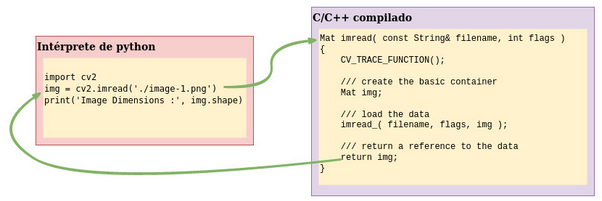
\includegraphics[width=8cm]{extender}
\end{figure}

\begin{figure}[h]
\caption{Embeber el intérprete}
\label{fig:embeber}
\centering
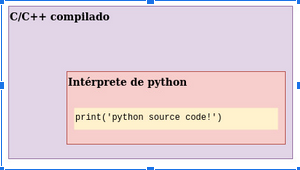
\includegraphics[width=4cm]{embeber}
\end{figure}

Cuando extendemos el intérprete, el programa principal es el intérprete de
Python que adquiere, a través de este mecanismo, la posibilidad de realizar
llamadas a módulos escritos en C/C++. Esto brinda principalmente dos
beneficios: por un lado, delegar parte de la computación en código de mejor
performance (procesamiento numérico, imágenes) y, por otro, la posibilidad de
realizar llamadas a las APIs del sistema en forma directa. Esta es una de las
formas en que muchos módulos propios de Python están escritos. \footnote{Ver por ejemplo
\url{https://github.com/python/cpython/tree/master/Modules})}

Cuando embebemos al intérprete, en cambio, el programa principal es otra
aplicación que usa al intérprete de Python como una librería más. Esta librería
tiene la capacidad de leer y ejecutar código fuente escrito en lenguaje Python.
Si bien se trata de un enfoque menos común, se puede utilizar como una manera
de agregar funcionalidad de scripting a sistemas escritos en C/C++ (por
ejemplo, configuración dinámica o elaboración de plugins). Notar que esto tiene
cierta afinidad con nuestro objetivo, que es lograr que una aplicación hecha en
C++ invoque código escrito en Python.

Para que el lector pueda tomar dimensión del nivel de dificultad que conlleva
la tarea de hacer que Python y C/C++ trabajen en conjunto (en cualquiera de las
dos direcciones) se brindan a continuación ejemplos de ambos tipos de
integración.

\paragraph{Extendiendo Python con C/C++}

Supongamos que queremos escribir en C una función que compute el cuadrado de un
número, y queremos que dicha función sea accesible al intérprete de Python.
Una implementación simple en C podría lucir así:

\inputminted{c}{codelistings/square.cc}

Nuestro objetivo sería poder escribir código Python como el siguiente:

\inputminted{Python}{codelistings/square_usage.py}

Cuando el código Python invoca la función square tienen que ocurrir tres cosas:

\begin{enumerate}
    \item El parámetro 2, que es un objeto Python debe ser convertido al tipo
    \verb!int!.

    \item El parámetro debe ser pasado a la función y el CPU debe ejecutar el
    código binario generado a partir del código fuente C.

    \item El valor de retorno (un \verb!int! con el valor 4) debe ser
    convertido a un objeto Python.
\end{enumerate}

Para comprender por qué esto es así, debemos recordar en primer lugar que
Python es un lenguaje interpretado. El código fuente debe ser convertido en una
serie de instrucciones para la máquina virtual de Python. En nuestro caso,
dichas instrucciones son:

\begin{minted}[linenos=false]{text}
1        0 LOAD_CONST               0 (0)
         2 LOAD_CONST               1 (None)
         4 IMPORT_NAME              0 (example)
         6 STORE_NAME               0 (example)

2        8 LOAD_NAME                1 (print)
        10 LOAD_CONST               2 (38)
        12 LOAD_NAME                0 (example)
        14 LOAD_METHOD              2 (square)
        16 LOAD_CONST               3 (2)
        18 CALL_METHOD              1
        20 BINARY_ADD
        22 CALL_FUNCTION            1
        24 POP_TOP
        26 LOAD_CONST               1 (None)
        28 RETURN_VALUE
\end{minted}

A continuación, esta serie de instrucciones son ejecutadas una a una. Esto es
muy diferente al código binario que genera una compilación de un archivo C.

Otra gran diferencia es que el valor 2 en Python es un objeto bastante más
complejo que en el mundo de C. En cPython, toda variable es una versión
especializada del tipo base que corresponde a \verb!PyObject!.

Entonces, la tarea de extender el intérprete con código hecho en C/C++ consiste
no sólo en escribir funcionalidad nueva en estos lenguajes, si no de realizar
todo el trabajo necesario para exponerlo al intérprete de Python.

El siguiente es un ejemplo completo de cómo sería la implementación de nuestro módulo. 

\inputminted{c}{codelistings/module.c}

Notar que la función \verb!square! ahora tiene los tipos que exporta el archivo
de encabezados \verb!Python.h!. Notar también que, además de la definición de
la función, se escribe código extra que representa la definición del módulo
donde esta función vive.

Si bien los detalles de compilación varían de acuerdo a las características del
sistema (lo cual no es relevante en este momento), así podríamos producir un
archivo \verb!example.so! que puede ser importado como librería desde el
intérprete:

\begin{minted}[linenos=false]{text}
# g++ -O3 -Wall -fPIC -I/usr/local/include -I/usr/include/Python3.6m -c example.cpp -o out.o
# g++ -shared out.o -L/usr/local/lib -o example.so

# Python3
>>> import example
>>> example.square(9)
81
\end{minted}

\paragraph{Intérprete embebido}

En este escenario el programa principal es una aplicación hecha en C/C++. Una
de las tareas de esta aplicación será la de inicializar (y finalizar) un
intérprete a través del cual pueda acceder a la funcionalidad desarrollada en
Python. El siguiente ejemplo, tomado de la documentación oficial, da muestra de
este enfoque. Supongamos que contamos con la siguiente definición de función
hecha en Python y almacenada en el archivo \verb!mul.py!:

\inputminted{Python}{codelistings/multiply.py}

El siguiente programa en C permitirá, una vez compilado, ejecutar dicho código:

\inputminted{c}{codelistings/use_multiply.c}

Para la compilación, los detalles varían de acuerdo a las características del
sistema, pero algo parecido a

\begin{minted}[linenos=false]{text}
# g++ -I/usr/include/Python3.6m -c cal.c
# g++ cal.o -lPython3.6m -o cal
\end{minted}

genera un binario llamado \verb!cal!, que permite hacer lo siguiente:

\begin{minted}[linenos=false]{text}
# ./cal mul multiply 12 4
Will compute 12 times 4
Result of call: 48
\end{minted}

Notar que la primera línea de salida proviene del archivo Python, mientras que
la segunda, del archivo C.

\paragraph{Extensiones e intérprete embebido en nuestro trabajo}

Ahora que contamos con marco de referencia para pensar las interacciones entre
C/C++ y Python, podemos plantearnos la pregunta: ¿cuál de los dos enfoques es
el apropiado para nuestro objetivo de extender \omnetpp{} usando Python?

Al extender (enfoque del tipo 1) el programa principal es el intérprete de
Python, que hace uso de código escrito en otro lenguaje. Al embeber el
intérprete (enfoque del tipo 2), el programa principal es escrito en C/C++ y se
encarga de inicializar (y también finalizar) un intérprete de Python para
acceder a funcionalidad escrita en este lenguaje. Sin duda, este último parece
más alineado con lo que queremos realizar. No obstante, ambos enfoques son
necesarios:

\begin{description}
    \item[Debemos extender el intérprete de Python] para que usuarios puedan heredar de \linebreak
    \verb!cSimpleModule! al especificar el funcionamiento de sus módulos. El
    sistema sólo acepta módulos que son subclases de aquella. Si esta tarea de
    especificación ha de realizarse en Python, como nos proponemos, entonces es
    menester habilitar la escritura de algo como
    \verb!from omnetpp import cSimpleModule!
    para comenzar a definir los módulos a partir de dicha clase base. Se sigue
    que al menos parte del código de \omnetpp{} debe ser expuesto al mundo de
    Python.

    \item[Debemos embeber el intérprete de Python en \omnetpp{}] para que la aplicación \linebreak
    principal siga siendo el binario de simulación que se obtiene al compilar
    un proyecto tradicional de \omnetpp{}. Si esto no fuera así, deberíamos
    reescribir, entre otras cosas, el código de la interfaz de usuario de las
    simulaciones.  Para conservar toda esa funcionalidad, queremos que el
    binario que genera \omnetpp{} cambie lo menos posible, pero que entre esos
    cambios se encuentre la capacidad de cargar módulos y ejecutar clases
    escritas en Python. Esto impone la necesidad de inicializar y finalizar un
    intérprete de Python (a su debido tiempo).
\end{description}

\begin{figure}[h]
\caption{Integrando \omnetpp{} con Python}
\label{fig:integrar}
\centering
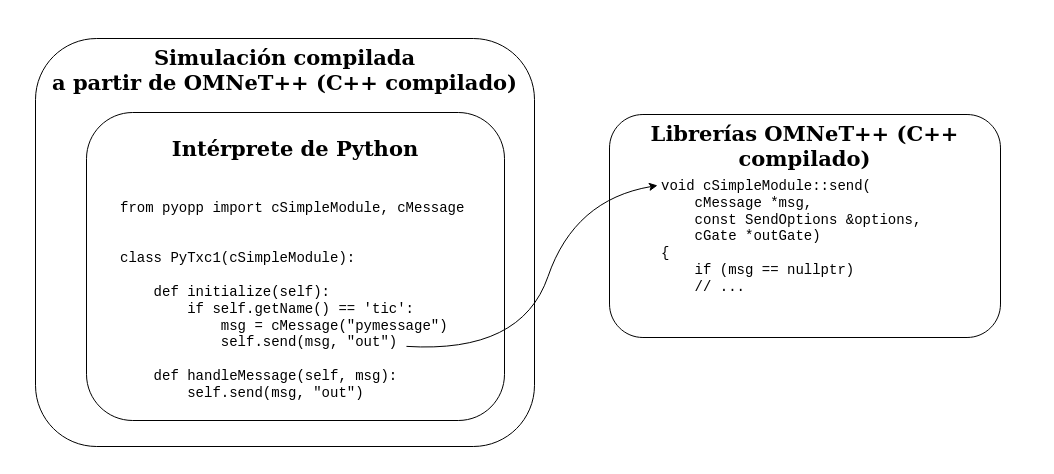
\includegraphics[width=\textwidth]{integrar}
\end{figure}

Esto plantea dos desafíos, que son el núcleo del trabajo realizado:

\begin{enumerate}
    \item ¿Cómo exponer al intérprete de Python toda la funcionalidad
    preexistente en las librerías de simulación, para que el usuario pueda
    escribir módulos simples en Python?

    \item ¿Cómo intervenir el proyecto \omnetpp{} de forma que instancie y
    ejecute un intérprete de Python embebido en él?
\end{enumerate}

\subsection{Herramientas de más alto nivel para lograr la integración}

Como se aprecia en los ejemplos de código provistos hasta el momento (extensión
e intérprete embebido), la tarea dista de ser trivial, a pesar de tratarse
apenas de funciones pequeñas con argumentos de tipos básicos. Es de esperar
grados de complejidad mucho mayores cuando el código involucre estructuras más
sofisticadas del lenguaje (funciones con número variable de argumentos,
argumentos con nombre, argumentos con valor por defecto, manejo de errores y
excepciones, clases, etc.).

Por otro lado, a diferencia de lo hecho en el primer ejemplo, donde escribimos
una función ad-hoc con el sólo objetivo de exponerla en Python, muchas veces se
busca exponer en Python varios miles de líneas de código que nunca fueron
hechos con este objetivo en mente, donde cada función, cada clase, debe ser
envuelta con una capa que traduzca los argumentos con los tipos que envía el
``mundo'' de Python en argumentos de C++ y viceversa (con los valores de
retorno).

Un ejemplo de esta problemática puede encontrarse en la generación de los
bindings para Python de OpenCV (librería hecha en C++, especializada en
algoritmos de procesamiento de imágenes). En How OpenCV-Python bindings are
generated?
\footnote{\url{https://docs.opencv.org/master/da/d49/tutorial_py_bindings_basics.html}}
leemos:

\begin{quotation}
In OpenCV, all algorithms are implemented in C++. But these algorithms can be
used from different languages like Python, Java etc. This is made possible by
the bindings generators. These generators create a bridge between C++ and
Python which enables users to call C++ functions from Python. (...)  So
extending all functions in OpenCV to Python by writing their wrapper functions
manually is a time-consuming task. So OpenCV does it in a more intelligent way.
OpenCV generates these wrapper functions automatically from the C++ headers
using some Python scripts (...)
\end{quotation}

En particular, el proyecto OpenCV resuelve el problema mediante scripts propios
que a partir de los archivos de encabezado de C++ pueden producir el código
necesario para exponer las clases y funciones al intérprete. 

Existen en el ecosistema de la creación de bindings y wrappers varios proyectos
que buscan resolver este problema de forma más genérica. Algunos de ellos son:

\begin{itemize}
    \item swig (\url{http://swig.org}): herramienta para la generación de
    código mediante el cual se puede conectar una aplicación hecha en C o C++
    con una variedad de lenguajes de programación. Típicamente se utiliza para
    parsear el código en C o C++ y proveer el código necesario para exponerlo
    en el lenguaje de destino.

    \item boost
    (\url{https://www.boost.org/doc/libs/1_77_0/libs/python/doc}):
    librería hecha en C++ con el objetivo de proveer integración entre C++ y
    Python. Facilita la tarea de exponer proyectos hechos en C++ como módulos
    de Python disminuyendo la cantidad de código que el usuario debe escribir
    para generar los bindings. Hay que mencionar que es una pequeña parte de un
    proyecto mucho más abarcativo formado por numerosas librerías para C++.

    \item pybind11 (\url{https://pybind11.readthedocs.io/en/stable/}): Comparte
    el objetivo (y mucha de la sintaxis) con boost.Python.  Intenta
    diferenciarse de aquella en que es una librería formada enteramente por
    encabezados (archivos .h). Su código es más escueto y en ocasiones permite
    simplificar la sintaxis en relación a boost.Python. 

    \item binder (\url{https://cppbinder.readthedocs.io/en/latest/about.html}):
    Intenta solucionar la generación automática del código necesario para
    exponer C++ a Python utilizando la librería pybind11.

    \item cpppy (\url{https://cppyy.readthedocs.io/en/latest/}): Haciendo uso
    de las librerías del proyecto LLVM permite ejecutar código C++ desde Python
    sin la necesidad de generación previa de bindings ni del uso de un lenguaje
    intermedio. El código en C++ se provee directamente como strings a
    funciones que producen LLVM IR (LLVM Intermediate Representation, una
    especie de assembly que usa LLVM antes de pasar a código máquina de una
    arquitectura específica) y se compila en tiempo de ejecución
    \cite{lavrijsen}.
\end{itemize}

Para dar idea al lector del tipo de beneficio que se obtiene al emplear estas
herramientas, se provee a continuación una reimplementación del segundo ejemplo
(embeber el intérprete) utilizando pybind11.

Recordemos que tenemos la siguiente definición de función en Python, en el
archivo mul.py

\inputminted{Python}{codelistings/multiply.py}

El siguiente código en C++, en el archivo cal.cpp

\inputminted{c}{codelistings/use_multiply_pybind.c}

puede ser compilado con

\begin{minted}[linenos=false]{text}
# g++ -O3 -Wall -std=c++11 -fPIC `Python3 -m pybind11 --includes` cal.cpp -o cal -lPython3.6m
\end{minted}

y ejecutado

\begin{minted}[linenos=false]{text}
# ./cal
Will compute 12 times 3
Result is 36
\end{minted}

obteniendo los mismos resultados que antes, pero con un código muchísimo más
escueto y sencillo.

Se eligió la herramienta pybind11 para lograr la interacción entre Python y C++
por resultar la más sencilla de utilizar y por ser su documentación muy
completa. Por otro lado, como se puede apreciar en el repositorio oficial
\footnote{\url{https://github.com/pybind/pybind11}}, resulta ser un proyecto
activamente mantenido y con mucho uso en la comunidad.

Si bien resulta muy atractivo el proyecto binder y su promesa de generar
código para exponer el proyecto usando pybind11 de forma automática, el
objetivo de este trabajo no fue nunca la automatización del proceso de
escritura de las librerías, si no encontrar una manera de extender \omnetpp{}
utilizando Python.

El proyecto cpppy resulta muy atractivo por el hecho de no tener que escribir
código intermedio alguno, pero al momento de este trabajo parece tener poca
actividad y su documentación no es tan clara y extensa.

\subsection{Entorno de trabajo}

La primera etapa del trabajo consistió en familiarizarse con el código de
\omnetpp{}. Para ello se procedió a descargar su código fuente del repositorio
público que se encuentra en github. Al momento de comenzar el trabajo, la
última versión estable era la 5.5.1.

Una vez obtenido el código fuente, se procedió a la compilación del mismo. Para
ello se siguieron las instrucciones provistas en la documentación del proyecto
y en numerosas fuentes web.

Para facilitar la repetición de esta experiencia (así como el uso de la versión
modificada de \omnetpp{} que permitiera una integración con Python) se utilizó
desde un principio el desarrollo dentro de contenedores Docker. Se procedió a
la definición de una imagen base que tuviera todas las dependencias de \omnetpp{}
preinstaladas y que permitiera fijar la versión de todos y cada uno de los
componentes involucrados (compilador, librerías, Python, etc.). Esta fue una
decisión muy acertada que permitió no sólo la repetibilidad de los resultados,
si no también minimizar posibles fuentes de error o incertidumbre dado el
control casi total del entorno de desarrollo.

\paragraph{Herramientas y versiones}

El siguiente es un listado de los principales componentes de software que
intervinieron en el desarrollo de este trabajo:

\begin{itemize}
    \item \omnetpp{} 5.5.1

    \item Linux 1902cc2cffcf 5.3.0-29-generic

    \item Ubuntu 18-10 (Cosmic)

    \item g++ (Ubuntu 8.3.0-6ubuntu1~18.10.1) 8.3.0

    \item GNU Make 4.2.1

    \item Python 3.6.8

    \item pybind11 2.4.3
\end{itemize}

En una etapa final del proyecto se diseñaron mecanismos para probar nuestro
código contra distintas versiones de \omnetpp{} y se comenzó a utilizar Ubuntu
19.10 con Python 3.7.5, sin dificultades observables.

\subsection{Caso de estudio}
La documentación oficial de \omnetpp{} provee un tutorial en siete partes que
va complejizando gradualmente una simulación llamada ``tictoc''
\footnote{\url{https://docs.omnetpp.org/tutorials/tictoc/}}. De esta forma se
busca que los nuevos usuarios puedan familiarizarse con las funcionalidades
principales que ofrece la herramienta.

La simulación ``tictoc'' (si bien conoce variaciones a lo largo del tutorial)
consiste esencialmente en una red con dos módulos (llamados tic y toc) que
intercambian un mismo mensaje ad infinitum (ver fig.~\ref{fig:tictoc}).

\begin{figure}[h]
\caption{Ejecución gráfica de la simulación ``tictoc''.}
\label{fig:tictoc}
\centering
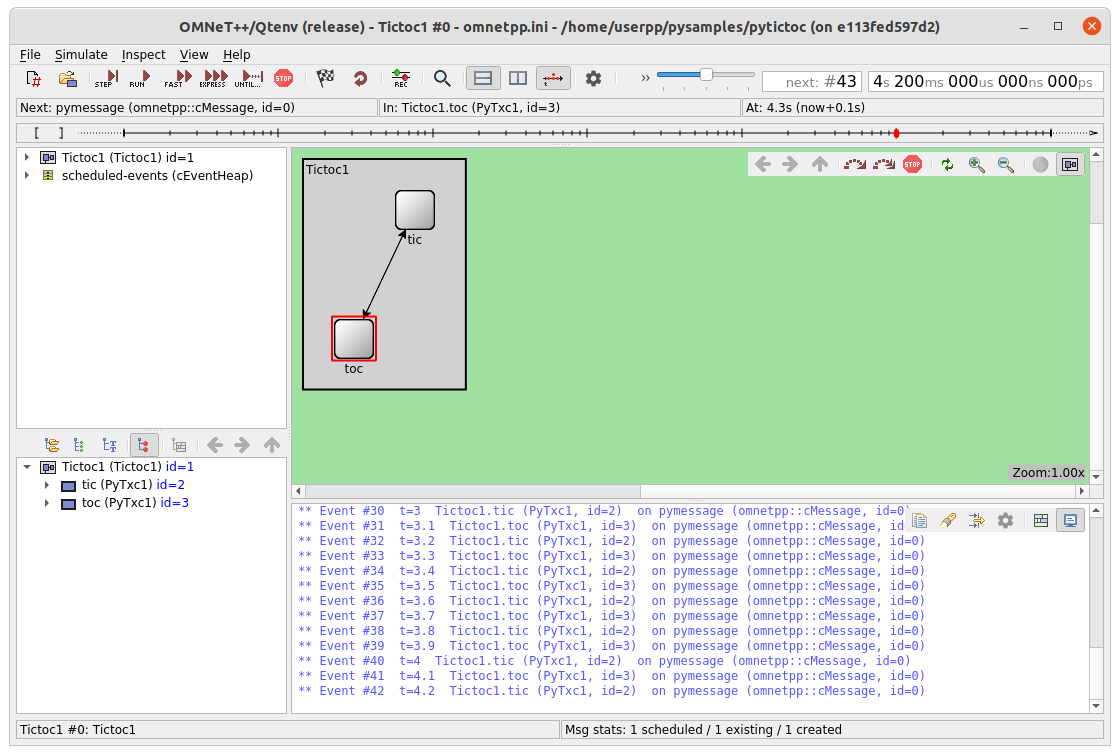
\includegraphics[width=\textwidth]{tictoc}
\end{figure}

Por la sencillez inicial y la complejidad incremental de esta simulación, se
usó como guía de todas las pruebas. Se estableció como primer objetivo poder
escribir los módulos del tutorial tictoc en Python. Esto permitió concentrarse
en las necesidades generales que permitieran la integración funcional de
\omnetpp{} con las clases escritas en Python.

Sólo una vez que se consiguió el objetivo primario, se prosiguió ampliando la
integración para permitir la implementación de módulos de mayor complejidad. En
una segunda etapa, la mayoría de las muestras en el directorio samples fueron
portadas a Python. Asimismo, se implementaron en Python algunos trabajos
prácticos de la cátedra Redes y Sistemas Distribuidos de FaMAF.
